\documentclass[twoside]{book}

% Packages required by doxygen
\usepackage{fixltx2e}
\usepackage{calc}
\usepackage{doxygen}
\usepackage[export]{adjustbox} % also loads graphicx
\usepackage{graphicx}
\usepackage[utf8]{inputenc}
\usepackage{makeidx}
\usepackage{multicol}
\usepackage{multirow}
\PassOptionsToPackage{warn}{textcomp}
\usepackage{textcomp}
\usepackage[nointegrals]{wasysym}
\usepackage[table]{xcolor}

% Font selection
\usepackage[T1]{fontenc}
\usepackage[scaled=.90]{helvet}
\usepackage{courier}
\usepackage{amssymb}
\usepackage{sectsty}
\renewcommand{\familydefault}{\sfdefault}
\allsectionsfont{%
  \fontseries{bc}\selectfont%
  \color{darkgray}%
}
\renewcommand{\DoxyLabelFont}{%
  \fontseries{bc}\selectfont%
  \color{darkgray}%
}
\newcommand{\+}{\discretionary{\mbox{\scriptsize$\hookleftarrow$}}{}{}}

% Page & text layout
\usepackage{geometry}
\geometry{%
  a4paper,%
  top=2.5cm,%
  bottom=2.5cm,%
  left=2.5cm,%
  right=2.5cm%
}
\tolerance=750
\hfuzz=15pt
\hbadness=750
\setlength{\emergencystretch}{15pt}
\setlength{\parindent}{0cm}
\setlength{\parskip}{3ex plus 2ex minus 2ex}
\makeatletter
\renewcommand{\paragraph}{%
  \@startsection{paragraph}{4}{0ex}{-1.0ex}{1.0ex}{%
    \normalfont\normalsize\bfseries\SS@parafont%
  }%
}
\renewcommand{\subparagraph}{%
  \@startsection{subparagraph}{5}{0ex}{-1.0ex}{1.0ex}{%
    \normalfont\normalsize\bfseries\SS@subparafont%
  }%
}
\makeatother

% Headers & footers
\usepackage{fancyhdr}
\pagestyle{fancyplain}
\fancyhead[LE]{\fancyplain{}{\bfseries\thepage}}
\fancyhead[CE]{\fancyplain{}{}}
\fancyhead[RE]{\fancyplain{}{\bfseries\leftmark}}
\fancyhead[LO]{\fancyplain{}{\bfseries\rightmark}}
\fancyhead[CO]{\fancyplain{}{}}
\fancyhead[RO]{\fancyplain{}{\bfseries\thepage}}
\fancyfoot[LE]{\fancyplain{}{}}
\fancyfoot[CE]{\fancyplain{}{}}
\fancyfoot[RE]{\fancyplain{}{\bfseries\scriptsize Generated by Doxygen }}
\fancyfoot[LO]{\fancyplain{}{\bfseries\scriptsize Generated by Doxygen }}
\fancyfoot[CO]{\fancyplain{}{}}
\fancyfoot[RO]{\fancyplain{}{}}
\renewcommand{\footrulewidth}{0.4pt}
\renewcommand{\chaptermark}[1]{%
  \markboth{#1}{}%
}
\renewcommand{\sectionmark}[1]{%
  \markright{\thesection\ #1}%
}

% Indices & bibliography
\usepackage{natbib}
\usepackage[titles]{tocloft}
\setcounter{tocdepth}{3}
\setcounter{secnumdepth}{5}
\makeindex

% Hyperlinks (required, but should be loaded last)
\usepackage{ifpdf}
\ifpdf
  \usepackage[pdftex,pagebackref=true]{hyperref}
\else
  \usepackage[ps2pdf,pagebackref=true]{hyperref}
\fi
\hypersetup{%
  colorlinks=true,%
  linkcolor=blue,%
  citecolor=blue,%
  unicode%
}

% Custom commands
\newcommand{\clearemptydoublepage}{%
  \newpage{\pagestyle{empty}\cleardoublepage}%
}

\usepackage{caption}
\captionsetup{labelsep=space,justification=centering,font={bf},singlelinecheck=off,skip=4pt,position=top}

%===== C O N T E N T S =====

\begin{document}

% Titlepage & ToC
\hypersetup{pageanchor=false,
             bookmarksnumbered=true,
             pdfencoding=unicode
            }
\pagenumbering{alph}
\begin{titlepage}
\vspace*{7cm}
\begin{center}%
{\Large Distancia\+\_\+de\+\_\+\+Levenshtein }\\
\vspace*{1cm}
{\large Generated by Doxygen 1.8.12}\\
\end{center}
\end{titlepage}
\clearemptydoublepage
\pagenumbering{roman}
\tableofcontents
\clearemptydoublepage
\pagenumbering{arabic}
\hypersetup{pageanchor=true}

%--- Begin generated contents ---
\chapter{Distancia Levenshtein}
\label{md__r_e_a_d_m_e}
\hypertarget{md__r_e_a_d_m_e}{}
\subsection*{Descripción\+:}

La {\bfseries Distancia de Levenshtein}, {\bfseries Distancia de Edición} o {\bfseries Distancia entre palabras} es el número mínimo de operaciones requeridas para transformar una \href{https://es.wikipedia.org/wiki/Cadena_de_caracteres}{\tt cadena de caracteres} en otra, se usa ampliamente en \href{https://es.wikipedia.org/wiki/Teor%C3%ADa_de_la_informaci%C3%B3n}{\tt teoría de la información} y \href{https://es.wikipedia.org/wiki/Ciencias_de_la_computaci%C3%B3n}{\tt ciencias de la computación}. Se entiende por operación, bien una inserción, eliminación o la sustitución de un carácter. Esta distancia recibe ese nombre en honor al científico ruso \href{https://es.wikipedia.org/wiki/Vlad%C3%ADmir_Levensht%C3%A9in}{\tt Vladimir Levenshtein}, quien se ocupó de esta distancia en 1965. Es útil en programas que determinan cuán similares son dos cadenas de caracteres, como es el caso de los correctores de ortografía.

Por ejemplo, la distancia de Levenshtein entre \char`\"{}casa\char`\"{} y \char`\"{}calle\char`\"{} es de 3 porque se necesitan al menos tres ediciones elementales para cambiar uno en el otro.


\begin{DoxyItemize}
\item casa → cala (sustitución de \textquotesingle{}s\textquotesingle{} por \textquotesingle{}l\textquotesingle{})
\item cala → calla (inserción de \textquotesingle{}l\textquotesingle{} entre \textquotesingle{}l\textquotesingle{} y \textquotesingle{}a\textquotesingle{})
\item calla → calle (sustitución de \textquotesingle{}a\textquotesingle{} por \textquotesingle{}e\textquotesingle{})
\end{DoxyItemize}

Se le considera una generalización de la \href{https://es.wikipedia.org/wiki/Distancia_de_Hamming}{\tt distancia de Hamming}, que se usa para cadenas de la misma longitud y que solo considera como operación la sustitución. Hay otras generalizaciones de la distancia de Levenshtein, como la \href{https://es.wikipedia.org/wiki/Distancia_de_Damerau-Levenshtein}{\tt distancia de Damerau-\/\+Levenshtein}, que consideran el intercambio de dos caracteres como una operación.

Como buena \char`\"{}distancia\char`\"{}, cumple (aunque es complicado demostrarlo formalmente), que\+:


\begin{DoxyItemize}
\item Dist(\+A,\+B) == Dist(\+B,\+A)
\item Dist(\+A,\+B) + Dist(\+B,\+C) $>$= Dist(\+A,\+C)
\end{DoxyItemize}

\subsection*{El Algoritmo\+:}

Se trata de un \href{https://es.wikipedia.org/wiki/Algoritmo}{\tt algoritmo} de tipo bottom-\/up, común en \href{https://es.wikipedia.org/wiki/Programaci%C3%B3n_din%C3%A1mica}{\tt programación dinámica}. Se apoya en el uso de una matriz (n + 1) × (m + 1), donde n y m son las longitudes de las cadenas. Aquí se indica el algoritmo en \href{https://es.wikipedia.org/wiki/Pseudoc%C3%B3digo}{\tt pseudocódigo} para una función Levenshtein\+Distance que toma dos cadenas, str1 de longitud len\+Str1, y str2 de longitud len\+Str2, y calcula la distancia Levenshtein entre ellos\+: \begin{DoxyVerb}int LevenshteinDistance(char str1[1..lenStr1], char str2[1..lenStr2])
    // d is a table with lenStr1+1 rows and lenStr2+1 columns
    declare int d[0..lenStr1, 0..lenStr2]
    // i and j are used to iterate over str1 and str2
    declare int i, j, cost

    for i from 0 to lenStr1
        d[i, 0] := i
    for j from 0 to lenStr2
        d[0, j] := j

    for i from 1 to lenStr1
        for j from 1 to lenStr2
            if str1[i-1] = str2[j-1]
                then cost := 0
            else
                cost := 1

            d[i, j] := minimum( d[i-1, j] + 1,      // deletion
                                d[i, j-1] + 1,      // insertion
                                d[i-1, j-1] + cost  // substitution
                                )
    return d[lenStr1, lenStr2]
\end{DoxyVerb}


\subsection*{Aplicaciones\+:}


\begin{DoxyItemize}
\item El proyecto A\+S\+JP usa la distancia de Levenshtein total en una lista de palabras en diferentes lenguas del mundo, para medir la \char`\"{}similaridad\char`\"{} o \char`\"{}cercanía\char`\"{} de las mismas, esa distancia calculada puede emplearse para proponer una clasificación filogenética tentativa de las lenguas del mundo.
\item La distancia de Damerau-\/\+Levenshtein es una generalización de la distancia de Levenshtein usada por los correctores ortográficos y en la detección de fraudes en listas de datos. 
\end{DoxyItemize}
\chapter{Namespace Index}
\section{Packages}
Here are the packages with brief descriptions (if available)\+:\begin{DoxyCompactList}
\item\contentsline{section}{\hyperlink{namespaceclases}{clases} }{\pageref{namespaceclases}}{}
\item\contentsline{section}{\hyperlink{namespaceclases_1_1_distancia_levenshtein}{clases.\+Distancia\+Levenshtein} }{\pageref{namespaceclases_1_1_distancia_levenshtein}}{}
\end{DoxyCompactList}

\chapter{Hierarchical Index}
\section{Class Hierarchy}
This inheritance list is sorted roughly, but not completely, alphabetically\+:\begin{DoxyCompactList}
\item \contentsline{section}{clases.\+Distancia\+Levenshtein.\+All\+Tests}{\pageref{classclases_1_1_distancia_levenshtein_1_1_all_tests}}{}
\item \contentsline{section}{clases.\+Distancia\+Levenshtein.\+App}{\pageref{classclases_1_1_distancia_levenshtein_1_1_app}}{}
\item \contentsline{section}{clases.\+Distancia\+Levenshtein.\+Levenshtein\+Distance}{\pageref{classclases_1_1_distancia_levenshtein_1_1_levenshtein_distance}}{}
\item \contentsline{section}{clases.\+Distancia\+Levenshtein.\+Levenshtein\+Distance\+Test01}{\pageref{classclases_1_1_distancia_levenshtein_1_1_levenshtein_distance_test01}}{}
\item \contentsline{section}{clases.\+Distancia\+Levenshtein.\+Levenshtein\+Distance\+Test02}{\pageref{classclases_1_1_distancia_levenshtein_1_1_levenshtein_distance_test02}}{}
\item \contentsline{section}{clases.\+Distancia\+Levenshtein.\+Levenshtein\+Distance\+Test03}{\pageref{classclases_1_1_distancia_levenshtein_1_1_levenshtein_distance_test03}}{}
\item \contentsline{section}{clases.\+Distancia\+Levenshtein.\+Levenshtein\+Distance\+Test04}{\pageref{classclases_1_1_distancia_levenshtein_1_1_levenshtein_distance_test04}}{}
\item Test\+Case\begin{DoxyCompactList}
\item \contentsline{section}{clases.\+Distancia\+Levenshtein.\+App\+Test}{\pageref{classclases_1_1_distancia_levenshtein_1_1_app_test}}{}
\end{DoxyCompactList}
\end{DoxyCompactList}

\chapter{Class Index}
\section{Class List}
Here are the classes, structs, unions and interfaces with brief descriptions\+:\begin{DoxyCompactList}
\item\contentsline{section}{\hyperlink{classclases_1_1_distancia_levenshtein_1_1_all_tests}{clases.\+Distancia\+Levenshtein.\+All\+Tests} \\*All\+Test de la Distancia de Levenshtein }{\pageref{classclases_1_1_distancia_levenshtein_1_1_all_tests}}{}
\item\contentsline{section}{\hyperlink{classclases_1_1_distancia_levenshtein_1_1_app}{clases.\+Distancia\+Levenshtein.\+App} \\*Clase Principal }{\pageref{classclases_1_1_distancia_levenshtein_1_1_app}}{}
\item\contentsline{section}{\hyperlink{classclases_1_1_distancia_levenshtein_1_1_app_test}{clases.\+Distancia\+Levenshtein.\+App\+Test} }{\pageref{classclases_1_1_distancia_levenshtein_1_1_app_test}}{}
\item\contentsline{section}{\hyperlink{classclases_1_1_distancia_levenshtein_1_1_levenshtein_distance}{clases.\+Distancia\+Levenshtein.\+Levenshtein\+Distance} \\*Clase que implementa la Distancia de Levenshtein }{\pageref{classclases_1_1_distancia_levenshtein_1_1_levenshtein_distance}}{}
\item\contentsline{section}{\hyperlink{classclases_1_1_distancia_levenshtein_1_1_levenshtein_distance_test01}{clases.\+Distancia\+Levenshtein.\+Levenshtein\+Distance\+Test01} \\*Test01 de la Distancia de Levenshtein }{\pageref{classclases_1_1_distancia_levenshtein_1_1_levenshtein_distance_test01}}{}
\item\contentsline{section}{\hyperlink{classclases_1_1_distancia_levenshtein_1_1_levenshtein_distance_test02}{clases.\+Distancia\+Levenshtein.\+Levenshtein\+Distance\+Test02} \\*Test02 de la Distancia de Levenshtein }{\pageref{classclases_1_1_distancia_levenshtein_1_1_levenshtein_distance_test02}}{}
\item\contentsline{section}{\hyperlink{classclases_1_1_distancia_levenshtein_1_1_levenshtein_distance_test03}{clases.\+Distancia\+Levenshtein.\+Levenshtein\+Distance\+Test03} \\*Test03 de la Distancia de Levenshtein }{\pageref{classclases_1_1_distancia_levenshtein_1_1_levenshtein_distance_test03}}{}
\item\contentsline{section}{\hyperlink{classclases_1_1_distancia_levenshtein_1_1_levenshtein_distance_test04}{clases.\+Distancia\+Levenshtein.\+Levenshtein\+Distance\+Test04} \\*Test04 de la Distancia de Levenshtein }{\pageref{classclases_1_1_distancia_levenshtein_1_1_levenshtein_distance_test04}}{}
\end{DoxyCompactList}

\chapter{File Index}
\section{File List}
Here is a list of all files with brief descriptions\+:\begin{DoxyCompactList}
\item\contentsline{section}{src/main/java/clases/\+Distancia\+Levenshtein/\hyperlink{_app_8java}{App.\+java} }{\pageref{_app_8java}}{}
\item\contentsline{section}{src/main/java/clases/\+Distancia\+Levenshtein/\hyperlink{_levenshtein_distance_8java}{Levenshtein\+Distance.\+java} }{\pageref{_levenshtein_distance_8java}}{}
\item\contentsline{section}{src/test/java/clases/\+Distancia\+Levenshtein/\hyperlink{_all_tests_8java}{All\+Tests.\+java} }{\pageref{_all_tests_8java}}{}
\item\contentsline{section}{src/test/java/clases/\+Distancia\+Levenshtein/\hyperlink{_app_test_8java}{App\+Test.\+java} }{\pageref{_app_test_8java}}{}
\item\contentsline{section}{src/test/java/clases/\+Distancia\+Levenshtein/\hyperlink{_levenshtein_distance_test01_8java}{Levenshtein\+Distance\+Test01.\+java} }{\pageref{_levenshtein_distance_test01_8java}}{}
\item\contentsline{section}{src/test/java/clases/\+Distancia\+Levenshtein/\hyperlink{_levenshtein_distance_test02_8java}{Levenshtein\+Distance\+Test02.\+java} }{\pageref{_levenshtein_distance_test02_8java}}{}
\item\contentsline{section}{src/test/java/clases/\+Distancia\+Levenshtein/\hyperlink{_levenshtein_distance_test03_8java}{Levenshtein\+Distance\+Test03.\+java} }{\pageref{_levenshtein_distance_test03_8java}}{}
\item\contentsline{section}{src/test/java/clases/\+Distancia\+Levenshtein/\hyperlink{_levenshtein_distance_test04_8java}{Levenshtein\+Distance\+Test04.\+java} }{\pageref{_levenshtein_distance_test04_8java}}{}
\end{DoxyCompactList}

\chapter{Namespace Documentation}
\hypertarget{namespaceclases}{}\section{Package clases}
\label{namespaceclases}\index{clases@{clases}}
\subsection*{Packages}
\begin{DoxyCompactItemize}
\item 
package \hyperlink{namespaceclases_1_1_distancia_levenshtein}{Distancia\+Levenshtein}
\end{DoxyCompactItemize}

\hypertarget{namespaceclases_1_1_distancia_levenshtein}{}\section{Package clases.\+Distancia\+Levenshtein}
\label{namespaceclases_1_1_distancia_levenshtein}\index{clases.\+Distancia\+Levenshtein@{clases.\+Distancia\+Levenshtein}}
\subsection*{Classes}
\begin{DoxyCompactItemize}
\item 
class \hyperlink{classclases_1_1_distancia_levenshtein_1_1_all_tests}{All\+Tests}
\item 
class \hyperlink{classclases_1_1_distancia_levenshtein_1_1_app}{App}
\item 
class \hyperlink{classclases_1_1_distancia_levenshtein_1_1_app_test}{App\+Test}
\item 
class \hyperlink{classclases_1_1_distancia_levenshtein_1_1_levenshtein_distance}{Levenshtein\+Distance}
\item 
class \hyperlink{classclases_1_1_distancia_levenshtein_1_1_levenshtein_distance_test01}{Levenshtein\+Distance\+Test01}
\item 
class \hyperlink{classclases_1_1_distancia_levenshtein_1_1_levenshtein_distance_test02}{Levenshtein\+Distance\+Test02}
\item 
class \hyperlink{classclases_1_1_distancia_levenshtein_1_1_levenshtein_distance_test03}{Levenshtein\+Distance\+Test03}
\item 
class \hyperlink{classclases_1_1_distancia_levenshtein_1_1_levenshtein_distance_test04}{Levenshtein\+Distance\+Test04}
\end{DoxyCompactItemize}

\chapter{Class Documentation}
\hypertarget{classclases_1_1_distancia_levenshtein_1_1_all_tests}{}\section{clases.\+Distancia\+Levenshtein.\+All\+Tests Class Reference}
\label{classclases_1_1_distancia_levenshtein_1_1_all_tests}\index{clases.\+Distancia\+Levenshtein.\+All\+Tests@{clases.\+Distancia\+Levenshtein.\+All\+Tests}}


All\+Test de la Distancia de Levenshtein.  




\subsection{Detailed Description}
All\+Test de la Distancia de Levenshtein. 

\begin{DoxyAuthor}{Author}
Joel Perez Ramos 
\end{DoxyAuthor}


The documentation for this class was generated from the following file\+:\begin{DoxyCompactItemize}
\item 
src/test/java/clases/\+Distancia\+Levenshtein/\hyperlink{_all_tests_8java}{All\+Tests.\+java}\end{DoxyCompactItemize}

\hypertarget{classclases_1_1_distancia_levenshtein_1_1_app}{}\section{clases.\+Distancia\+Levenshtein.\+App Class Reference}
\label{classclases_1_1_distancia_levenshtein_1_1_app}\index{clases.\+Distancia\+Levenshtein.\+App@{clases.\+Distancia\+Levenshtein.\+App}}


Clase Principal.  


\subsection*{Static Public Member Functions}
\begin{DoxyCompactItemize}
\item 
static void \hyperlink{classclases_1_1_distancia_levenshtein_1_1_app_ac5da9898119949a7134b3a01f98be655}{main} (String\mbox{[}$\,$\mbox{]} args)
\begin{DoxyCompactList}\small\item\em Main. \end{DoxyCompactList}\end{DoxyCompactItemize}


\subsection{Detailed Description}
Clase Principal. 

\begin{DoxyAuthor}{Author}
Joel Perez Ramos 
\end{DoxyAuthor}


\subsection{Member Function Documentation}
\hypertarget{classclases_1_1_distancia_levenshtein_1_1_app_ac5da9898119949a7134b3a01f98be655}{}\label{classclases_1_1_distancia_levenshtein_1_1_app_ac5da9898119949a7134b3a01f98be655} 
\index{clases\+::\+Distancia\+Levenshtein\+::\+App@{clases\+::\+Distancia\+Levenshtein\+::\+App}!main@{main}}
\index{main@{main}!clases\+::\+Distancia\+Levenshtein\+::\+App@{clases\+::\+Distancia\+Levenshtein\+::\+App}}
\subsubsection{\texorpdfstring{main()}{main()}}
{\footnotesize\ttfamily static void clases.\+Distancia\+Levenshtein.\+App.\+main (\begin{DoxyParamCaption}\item[{String \mbox{[}$\,$\mbox{]}}]{args }\end{DoxyParamCaption})\hspace{0.3cm}{\ttfamily [static]}}



Main. 


\begin{DoxyParams}{Parameters}
{\em args} & \\
\hline
\end{DoxyParams}


The documentation for this class was generated from the following file\+:\begin{DoxyCompactItemize}
\item 
src/main/java/clases/\+Distancia\+Levenshtein/\hyperlink{_app_8java}{App.\+java}\end{DoxyCompactItemize}

\hypertarget{classclases_1_1_distancia_levenshtein_1_1_app_test}{}\section{clases.\+Distancia\+Levenshtein.\+App\+Test Class Reference}
\label{classclases_1_1_distancia_levenshtein_1_1_app_test}\index{clases.\+Distancia\+Levenshtein.\+App\+Test@{clases.\+Distancia\+Levenshtein.\+App\+Test}}
Inheritance diagram for clases.\+Distancia\+Levenshtein.\+App\+Test\+:\begin{figure}[H]
\begin{center}
\leavevmode
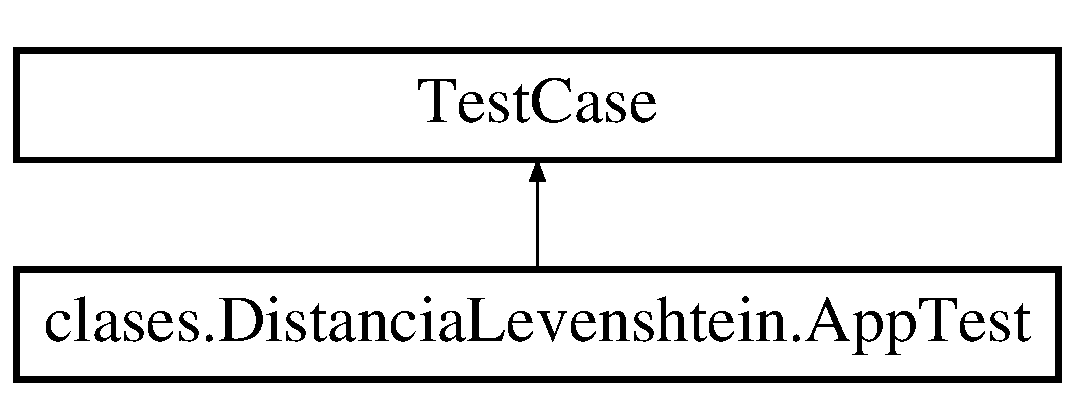
\includegraphics[height=2.000000cm]{classclases_1_1_distancia_levenshtein_1_1_app_test}
\end{center}
\end{figure}
\subsection*{Public Member Functions}
\begin{DoxyCompactItemize}
\item 
\hyperlink{classclases_1_1_distancia_levenshtein_1_1_app_test_a811706b4c4e90cf825130e5603ec8484}{App\+Test} (String test\+Name)
\item 
void \hyperlink{classclases_1_1_distancia_levenshtein_1_1_app_test_afe16cffbe326f0e959c29805ac205c90}{test\+App} ()
\end{DoxyCompactItemize}
\subsection*{Static Public Member Functions}
\begin{DoxyCompactItemize}
\item 
static Test \hyperlink{classclases_1_1_distancia_levenshtein_1_1_app_test_a2f8dab2e95f46b42a3b0b1836b283f53}{suite} ()
\end{DoxyCompactItemize}


\subsection{Detailed Description}
Unit test for simple \hyperlink{classclases_1_1_distancia_levenshtein_1_1_app}{App}. 

\subsection{Constructor \& Destructor Documentation}
\hypertarget{classclases_1_1_distancia_levenshtein_1_1_app_test_a811706b4c4e90cf825130e5603ec8484}{}\label{classclases_1_1_distancia_levenshtein_1_1_app_test_a811706b4c4e90cf825130e5603ec8484} 
\index{clases\+::\+Distancia\+Levenshtein\+::\+App\+Test@{clases\+::\+Distancia\+Levenshtein\+::\+App\+Test}!App\+Test@{App\+Test}}
\index{App\+Test@{App\+Test}!clases\+::\+Distancia\+Levenshtein\+::\+App\+Test@{clases\+::\+Distancia\+Levenshtein\+::\+App\+Test}}
\subsubsection{\texorpdfstring{App\+Test()}{AppTest()}}
{\footnotesize\ttfamily clases.\+Distancia\+Levenshtein.\+App\+Test.\+App\+Test (\begin{DoxyParamCaption}\item[{String}]{test\+Name }\end{DoxyParamCaption})}

Create the test case


\begin{DoxyParams}{Parameters}
{\em test\+Name} & name of the test case \\
\hline
\end{DoxyParams}


\subsection{Member Function Documentation}
\hypertarget{classclases_1_1_distancia_levenshtein_1_1_app_test_a2f8dab2e95f46b42a3b0b1836b283f53}{}\label{classclases_1_1_distancia_levenshtein_1_1_app_test_a2f8dab2e95f46b42a3b0b1836b283f53} 
\index{clases\+::\+Distancia\+Levenshtein\+::\+App\+Test@{clases\+::\+Distancia\+Levenshtein\+::\+App\+Test}!suite@{suite}}
\index{suite@{suite}!clases\+::\+Distancia\+Levenshtein\+::\+App\+Test@{clases\+::\+Distancia\+Levenshtein\+::\+App\+Test}}
\subsubsection{\texorpdfstring{suite()}{suite()}}
{\footnotesize\ttfamily static Test clases.\+Distancia\+Levenshtein.\+App\+Test.\+suite (\begin{DoxyParamCaption}{ }\end{DoxyParamCaption})\hspace{0.3cm}{\ttfamily [static]}}

\begin{DoxyReturn}{Returns}
the suite of tests being tested 
\end{DoxyReturn}
\hypertarget{classclases_1_1_distancia_levenshtein_1_1_app_test_afe16cffbe326f0e959c29805ac205c90}{}\label{classclases_1_1_distancia_levenshtein_1_1_app_test_afe16cffbe326f0e959c29805ac205c90} 
\index{clases\+::\+Distancia\+Levenshtein\+::\+App\+Test@{clases\+::\+Distancia\+Levenshtein\+::\+App\+Test}!test\+App@{test\+App}}
\index{test\+App@{test\+App}!clases\+::\+Distancia\+Levenshtein\+::\+App\+Test@{clases\+::\+Distancia\+Levenshtein\+::\+App\+Test}}
\subsubsection{\texorpdfstring{test\+App()}{testApp()}}
{\footnotesize\ttfamily void clases.\+Distancia\+Levenshtein.\+App\+Test.\+test\+App (\begin{DoxyParamCaption}{ }\end{DoxyParamCaption})}

Rigourous Test \+:-\/) 

The documentation for this class was generated from the following file\+:\begin{DoxyCompactItemize}
\item 
src/test/java/clases/\+Distancia\+Levenshtein/\hyperlink{_app_test_8java}{App\+Test.\+java}\end{DoxyCompactItemize}

\hypertarget{classclases_1_1_distancia_levenshtein_1_1_levenshtein_distance}{}\section{clases.\+Distancia\+Levenshtein.\+Levenshtein\+Distance Class Reference}
\label{classclases_1_1_distancia_levenshtein_1_1_levenshtein_distance}\index{clases.\+Distancia\+Levenshtein.\+Levenshtein\+Distance@{clases.\+Distancia\+Levenshtein.\+Levenshtein\+Distance}}


Clase que implementa la Distancia de Levenshtein.  


\subsection*{Static Public Member Functions}
\begin{DoxyCompactItemize}
\item 
static int \hyperlink{classclases_1_1_distancia_levenshtein_1_1_levenshtein_distance_a32fafec4e825f1e645f3edb717515098}{compute\+Levenshtein\+Distance} (String str1, String str2)
\begin{DoxyCompactList}\small\item\em Metodo que llama a la implementacion de la Distancia de Levenshtein. \end{DoxyCompactList}\end{DoxyCompactItemize}
\subsection*{Static Private Member Functions}
\begin{DoxyCompactItemize}
\item 
static int \hyperlink{classclases_1_1_distancia_levenshtein_1_1_levenshtein_distance_a670f5fdf074856d2fa62eaedb9b36cad}{minimum} (int a, int b, int c)
\begin{DoxyCompactList}\small\item\em Metodo que retorna el valor minimo de tres enteros. \end{DoxyCompactList}\item 
static int \hyperlink{classclases_1_1_distancia_levenshtein_1_1_levenshtein_distance_a5391113c57cf7ac23d8d7ab745a7e979}{compute\+Levenshtein\+Distance} (char\mbox{[}$\,$\mbox{]} str1, char\mbox{[}$\,$\mbox{]} str2)
\begin{DoxyCompactList}\small\item\em Metodo que implementa el algoritmo de la Distancia de Levenstein. \end{DoxyCompactList}\end{DoxyCompactItemize}


\subsection{Detailed Description}
Clase que implementa la Distancia de Levenshtein. 

\begin{DoxyAuthor}{Author}
Joel Perez Ramos 
\end{DoxyAuthor}


\subsection{Member Function Documentation}
\hypertarget{classclases_1_1_distancia_levenshtein_1_1_levenshtein_distance_a32fafec4e825f1e645f3edb717515098}{}\label{classclases_1_1_distancia_levenshtein_1_1_levenshtein_distance_a32fafec4e825f1e645f3edb717515098} 
\index{clases\+::\+Distancia\+Levenshtein\+::\+Levenshtein\+Distance@{clases\+::\+Distancia\+Levenshtein\+::\+Levenshtein\+Distance}!compute\+Levenshtein\+Distance@{compute\+Levenshtein\+Distance}}
\index{compute\+Levenshtein\+Distance@{compute\+Levenshtein\+Distance}!clases\+::\+Distancia\+Levenshtein\+::\+Levenshtein\+Distance@{clases\+::\+Distancia\+Levenshtein\+::\+Levenshtein\+Distance}}
\subsubsection{\texorpdfstring{compute\+Levenshtein\+Distance()}{computeLevenshteinDistance()}\hspace{0.1cm}{\footnotesize\ttfamily [1/2]}}
{\footnotesize\ttfamily static int clases.\+Distancia\+Levenshtein.\+Levenshtein\+Distance.\+compute\+Levenshtein\+Distance (\begin{DoxyParamCaption}\item[{String}]{str1,  }\item[{String}]{str2 }\end{DoxyParamCaption})\hspace{0.3cm}{\ttfamily [static]}}



Metodo que llama a la implementacion de la Distancia de Levenshtein. 


\begin{DoxyParams}{Parameters}
{\em str1} & \\
\hline
{\em str2} & \\
\hline
\end{DoxyParams}
\begin{DoxyReturn}{Returns}

\end{DoxyReturn}
\hypertarget{classclases_1_1_distancia_levenshtein_1_1_levenshtein_distance_a5391113c57cf7ac23d8d7ab745a7e979}{}\label{classclases_1_1_distancia_levenshtein_1_1_levenshtein_distance_a5391113c57cf7ac23d8d7ab745a7e979} 
\index{clases\+::\+Distancia\+Levenshtein\+::\+Levenshtein\+Distance@{clases\+::\+Distancia\+Levenshtein\+::\+Levenshtein\+Distance}!compute\+Levenshtein\+Distance@{compute\+Levenshtein\+Distance}}
\index{compute\+Levenshtein\+Distance@{compute\+Levenshtein\+Distance}!clases\+::\+Distancia\+Levenshtein\+::\+Levenshtein\+Distance@{clases\+::\+Distancia\+Levenshtein\+::\+Levenshtein\+Distance}}
\subsubsection{\texorpdfstring{compute\+Levenshtein\+Distance()}{computeLevenshteinDistance()}\hspace{0.1cm}{\footnotesize\ttfamily [2/2]}}
{\footnotesize\ttfamily static int clases.\+Distancia\+Levenshtein.\+Levenshtein\+Distance.\+compute\+Levenshtein\+Distance (\begin{DoxyParamCaption}\item[{char \mbox{[}$\,$\mbox{]}}]{str1,  }\item[{char \mbox{[}$\,$\mbox{]}}]{str2 }\end{DoxyParamCaption})\hspace{0.3cm}{\ttfamily [static]}, {\ttfamily [private]}}



Metodo que implementa el algoritmo de la Distancia de Levenstein. 


\begin{DoxyParams}{Parameters}
{\em str1} & \\
\hline
{\em str2} & \\
\hline
\end{DoxyParams}
\begin{DoxyReturn}{Returns}

\end{DoxyReturn}
\hypertarget{classclases_1_1_distancia_levenshtein_1_1_levenshtein_distance_a670f5fdf074856d2fa62eaedb9b36cad}{}\label{classclases_1_1_distancia_levenshtein_1_1_levenshtein_distance_a670f5fdf074856d2fa62eaedb9b36cad} 
\index{clases\+::\+Distancia\+Levenshtein\+::\+Levenshtein\+Distance@{clases\+::\+Distancia\+Levenshtein\+::\+Levenshtein\+Distance}!minimum@{minimum}}
\index{minimum@{minimum}!clases\+::\+Distancia\+Levenshtein\+::\+Levenshtein\+Distance@{clases\+::\+Distancia\+Levenshtein\+::\+Levenshtein\+Distance}}
\subsubsection{\texorpdfstring{minimum()}{minimum()}}
{\footnotesize\ttfamily static int clases.\+Distancia\+Levenshtein.\+Levenshtein\+Distance.\+minimum (\begin{DoxyParamCaption}\item[{int}]{a,  }\item[{int}]{b,  }\item[{int}]{c }\end{DoxyParamCaption})\hspace{0.3cm}{\ttfamily [static]}, {\ttfamily [private]}}



Metodo que retorna el valor minimo de tres enteros. 


\begin{DoxyParams}{Parameters}
{\em a} & \\
\hline
{\em b} & \\
\hline
{\em c} & \\
\hline
\end{DoxyParams}
\begin{DoxyReturn}{Returns}

\end{DoxyReturn}


The documentation for this class was generated from the following file\+:\begin{DoxyCompactItemize}
\item 
src/main/java/clases/\+Distancia\+Levenshtein/\hyperlink{_levenshtein_distance_8java}{Levenshtein\+Distance.\+java}\end{DoxyCompactItemize}

\hypertarget{classclases_1_1_distancia_levenshtein_1_1_levenshtein_distance_test01}{}\section{clases.\+Distancia\+Levenshtein.\+Levenshtein\+Distance\+Test01 Class Reference}
\label{classclases_1_1_distancia_levenshtein_1_1_levenshtein_distance_test01}\index{clases.\+Distancia\+Levenshtein.\+Levenshtein\+Distance\+Test01@{clases.\+Distancia\+Levenshtein.\+Levenshtein\+Distance\+Test01}}


Test01 de la Distancia de Levenshtein.  


\subsection*{Public Member Functions}
\begin{DoxyCompactItemize}
\item 
void \hyperlink{classclases_1_1_distancia_levenshtein_1_1_levenshtein_distance_test01_aae192451049290eabe6d0ac2e00f254b}{test\+Compute\+Levenshtein\+Distance} ()
\end{DoxyCompactItemize}


\subsection{Detailed Description}
Test01 de la Distancia de Levenshtein. 

\begin{DoxyAuthor}{Author}
Joel Perez Ramos 
\end{DoxyAuthor}


\subsection{Member Function Documentation}
\hypertarget{classclases_1_1_distancia_levenshtein_1_1_levenshtein_distance_test01_aae192451049290eabe6d0ac2e00f254b}{}\label{classclases_1_1_distancia_levenshtein_1_1_levenshtein_distance_test01_aae192451049290eabe6d0ac2e00f254b} 
\index{clases\+::\+Distancia\+Levenshtein\+::\+Levenshtein\+Distance\+Test01@{clases\+::\+Distancia\+Levenshtein\+::\+Levenshtein\+Distance\+Test01}!test\+Compute\+Levenshtein\+Distance@{test\+Compute\+Levenshtein\+Distance}}
\index{test\+Compute\+Levenshtein\+Distance@{test\+Compute\+Levenshtein\+Distance}!clases\+::\+Distancia\+Levenshtein\+::\+Levenshtein\+Distance\+Test01@{clases\+::\+Distancia\+Levenshtein\+::\+Levenshtein\+Distance\+Test01}}
\subsubsection{\texorpdfstring{test\+Compute\+Levenshtein\+Distance()}{testComputeLevenshteinDistance()}}
{\footnotesize\ttfamily void clases.\+Distancia\+Levenshtein.\+Levenshtein\+Distance\+Test01.\+test\+Compute\+Levenshtein\+Distance (\begin{DoxyParamCaption}{ }\end{DoxyParamCaption})}



The documentation for this class was generated from the following file\+:\begin{DoxyCompactItemize}
\item 
src/test/java/clases/\+Distancia\+Levenshtein/\hyperlink{_levenshtein_distance_test01_8java}{Levenshtein\+Distance\+Test01.\+java}\end{DoxyCompactItemize}

\hypertarget{classclases_1_1_distancia_levenshtein_1_1_levenshtein_distance_test02}{}\section{clases.\+Distancia\+Levenshtein.\+Levenshtein\+Distance\+Test02 Class Reference}
\label{classclases_1_1_distancia_levenshtein_1_1_levenshtein_distance_test02}\index{clases.\+Distancia\+Levenshtein.\+Levenshtein\+Distance\+Test02@{clases.\+Distancia\+Levenshtein.\+Levenshtein\+Distance\+Test02}}
\subsection*{Public Member Functions}
\begin{DoxyCompactItemize}
\item 
void \hyperlink{classclases_1_1_distancia_levenshtein_1_1_levenshtein_distance_test02_a0fb8d5113fa9cf3ce9f2378b06b3fdd7}{test\+Compute\+Levenshtein\+Distance} ()
\end{DoxyCompactItemize}


\subsection{Detailed Description}
Test02 de la Distancia de Levenshtein. \begin{DoxyAuthor}{Author}
Joel Perez Ramos 
\end{DoxyAuthor}


\subsection{Member Function Documentation}
\hypertarget{classclases_1_1_distancia_levenshtein_1_1_levenshtein_distance_test02_a0fb8d5113fa9cf3ce9f2378b06b3fdd7}{}\label{classclases_1_1_distancia_levenshtein_1_1_levenshtein_distance_test02_a0fb8d5113fa9cf3ce9f2378b06b3fdd7} 
\index{clases\+::\+Distancia\+Levenshtein\+::\+Levenshtein\+Distance\+Test02@{clases\+::\+Distancia\+Levenshtein\+::\+Levenshtein\+Distance\+Test02}!test\+Compute\+Levenshtein\+Distance@{test\+Compute\+Levenshtein\+Distance}}
\index{test\+Compute\+Levenshtein\+Distance@{test\+Compute\+Levenshtein\+Distance}!clases\+::\+Distancia\+Levenshtein\+::\+Levenshtein\+Distance\+Test02@{clases\+::\+Distancia\+Levenshtein\+::\+Levenshtein\+Distance\+Test02}}
\subsubsection{\texorpdfstring{test\+Compute\+Levenshtein\+Distance()}{testComputeLevenshteinDistance()}}
{\footnotesize\ttfamily void clases.\+Distancia\+Levenshtein.\+Levenshtein\+Distance\+Test02.\+test\+Compute\+Levenshtein\+Distance (\begin{DoxyParamCaption}{ }\end{DoxyParamCaption})}



The documentation for this class was generated from the following file\+:\begin{DoxyCompactItemize}
\item 
src/test/java/clases/\+Distancia\+Levenshtein/\hyperlink{_levenshtein_distance_test02_8java}{Levenshtein\+Distance\+Test02.\+java}\end{DoxyCompactItemize}

\hypertarget{classclases_1_1_distancia_levenshtein_1_1_levenshtein_distance_test03}{}\section{clases.\+Distancia\+Levenshtein.\+Levenshtein\+Distance\+Test03 Class Reference}
\label{classclases_1_1_distancia_levenshtein_1_1_levenshtein_distance_test03}\index{clases.\+Distancia\+Levenshtein.\+Levenshtein\+Distance\+Test03@{clases.\+Distancia\+Levenshtein.\+Levenshtein\+Distance\+Test03}}


Test03 de la Distancia de Levenshtein.  


\subsection*{Public Member Functions}
\begin{DoxyCompactItemize}
\item 
void \hyperlink{classclases_1_1_distancia_levenshtein_1_1_levenshtein_distance_test03_afa83a142e84686e31e74757c35a8db60}{test\+Compute\+Levenshtein\+Distance} ()
\end{DoxyCompactItemize}


\subsection{Detailed Description}
Test03 de la Distancia de Levenshtein. 

\begin{DoxyAuthor}{Author}
Joel Perez Ramos 
\end{DoxyAuthor}


\subsection{Member Function Documentation}
\hypertarget{classclases_1_1_distancia_levenshtein_1_1_levenshtein_distance_test03_afa83a142e84686e31e74757c35a8db60}{}\label{classclases_1_1_distancia_levenshtein_1_1_levenshtein_distance_test03_afa83a142e84686e31e74757c35a8db60} 
\index{clases\+::\+Distancia\+Levenshtein\+::\+Levenshtein\+Distance\+Test03@{clases\+::\+Distancia\+Levenshtein\+::\+Levenshtein\+Distance\+Test03}!test\+Compute\+Levenshtein\+Distance@{test\+Compute\+Levenshtein\+Distance}}
\index{test\+Compute\+Levenshtein\+Distance@{test\+Compute\+Levenshtein\+Distance}!clases\+::\+Distancia\+Levenshtein\+::\+Levenshtein\+Distance\+Test03@{clases\+::\+Distancia\+Levenshtein\+::\+Levenshtein\+Distance\+Test03}}
\subsubsection{\texorpdfstring{test\+Compute\+Levenshtein\+Distance()}{testComputeLevenshteinDistance()}}
{\footnotesize\ttfamily void clases.\+Distancia\+Levenshtein.\+Levenshtein\+Distance\+Test03.\+test\+Compute\+Levenshtein\+Distance (\begin{DoxyParamCaption}{ }\end{DoxyParamCaption})}



The documentation for this class was generated from the following file\+:\begin{DoxyCompactItemize}
\item 
src/test/java/clases/\+Distancia\+Levenshtein/\hyperlink{_levenshtein_distance_test03_8java}{Levenshtein\+Distance\+Test03.\+java}\end{DoxyCompactItemize}

\hypertarget{classclases_1_1_distancia_levenshtein_1_1_levenshtein_distance_test04}{}\section{clases.\+Distancia\+Levenshtein.\+Levenshtein\+Distance\+Test04 Class Reference}
\label{classclases_1_1_distancia_levenshtein_1_1_levenshtein_distance_test04}\index{clases.\+Distancia\+Levenshtein.\+Levenshtein\+Distance\+Test04@{clases.\+Distancia\+Levenshtein.\+Levenshtein\+Distance\+Test04}}
\subsection*{Public Member Functions}
\begin{DoxyCompactItemize}
\item 
void \hyperlink{classclases_1_1_distancia_levenshtein_1_1_levenshtein_distance_test04_a066861d7e72c8c5912e032286e892f67}{test\+Compute\+Levenshtein\+Distance} ()
\end{DoxyCompactItemize}


\subsection{Detailed Description}
Test04 de la Distancia de Levenshtein. \begin{DoxyAuthor}{Author}
Joey 
\end{DoxyAuthor}


\subsection{Member Function Documentation}
\hypertarget{classclases_1_1_distancia_levenshtein_1_1_levenshtein_distance_test04_a066861d7e72c8c5912e032286e892f67}{}\label{classclases_1_1_distancia_levenshtein_1_1_levenshtein_distance_test04_a066861d7e72c8c5912e032286e892f67} 
\index{clases\+::\+Distancia\+Levenshtein\+::\+Levenshtein\+Distance\+Test04@{clases\+::\+Distancia\+Levenshtein\+::\+Levenshtein\+Distance\+Test04}!test\+Compute\+Levenshtein\+Distance@{test\+Compute\+Levenshtein\+Distance}}
\index{test\+Compute\+Levenshtein\+Distance@{test\+Compute\+Levenshtein\+Distance}!clases\+::\+Distancia\+Levenshtein\+::\+Levenshtein\+Distance\+Test04@{clases\+::\+Distancia\+Levenshtein\+::\+Levenshtein\+Distance\+Test04}}
\subsubsection{\texorpdfstring{test\+Compute\+Levenshtein\+Distance()}{testComputeLevenshteinDistance()}}
{\footnotesize\ttfamily void clases.\+Distancia\+Levenshtein.\+Levenshtein\+Distance\+Test04.\+test\+Compute\+Levenshtein\+Distance (\begin{DoxyParamCaption}{ }\end{DoxyParamCaption})}



The documentation for this class was generated from the following file\+:\begin{DoxyCompactItemize}
\item 
src/test/java/clases/\+Distancia\+Levenshtein/\hyperlink{_levenshtein_distance_test04_8java}{Levenshtein\+Distance\+Test04.\+java}\end{DoxyCompactItemize}

\chapter{File Documentation}
\hypertarget{_r_e_a_d_m_e_8md}{}\section{R\+E\+A\+D\+M\+E.\+md File Reference}
\label{_r_e_a_d_m_e_8md}\index{R\+E\+A\+D\+M\+E.\+md@{R\+E\+A\+D\+M\+E.\+md}}

\hypertarget{_app_8java}{}\section{src/main/java/clases/\+Distancia\+Levenshtein/\+App.java File Reference}
\label{_app_8java}\index{src/main/java/clases/\+Distancia\+Levenshtein/\+App.\+java@{src/main/java/clases/\+Distancia\+Levenshtein/\+App.\+java}}
\subsection*{Classes}
\begin{DoxyCompactItemize}
\item 
class \hyperlink{classclases_1_1_distancia_levenshtein_1_1_app}{clases.\+Distancia\+Levenshtein.\+App}
\begin{DoxyCompactList}\small\item\em Clase Principal. \end{DoxyCompactList}\end{DoxyCompactItemize}
\subsection*{Packages}
\begin{DoxyCompactItemize}
\item 
package \hyperlink{namespaceclases_1_1_distancia_levenshtein}{clases.\+Distancia\+Levenshtein}
\end{DoxyCompactItemize}

\hypertarget{_levenshtein_distance_8java}{}\section{src/main/java/clases/\+Distancia\+Levenshtein/\+Levenshtein\+Distance.java File Reference}
\label{_levenshtein_distance_8java}\index{src/main/java/clases/\+Distancia\+Levenshtein/\+Levenshtein\+Distance.\+java@{src/main/java/clases/\+Distancia\+Levenshtein/\+Levenshtein\+Distance.\+java}}
\subsection*{Classes}
\begin{DoxyCompactItemize}
\item 
class \hyperlink{classclases_1_1_distancia_levenshtein_1_1_levenshtein_distance}{clases.\+Distancia\+Levenshtein.\+Levenshtein\+Distance}
\end{DoxyCompactItemize}
\subsection*{Packages}
\begin{DoxyCompactItemize}
\item 
package \hyperlink{namespaceclases_1_1_distancia_levenshtein}{clases.\+Distancia\+Levenshtein}
\end{DoxyCompactItemize}

\hypertarget{_all_tests_8java}{}\section{src/test/java/clases/\+Distancia\+Levenshtein/\+All\+Tests.java File Reference}
\label{_all_tests_8java}\index{src/test/java/clases/\+Distancia\+Levenshtein/\+All\+Tests.\+java@{src/test/java/clases/\+Distancia\+Levenshtein/\+All\+Tests.\+java}}
\subsection*{Classes}
\begin{DoxyCompactItemize}
\item 
class \hyperlink{classclases_1_1_distancia_levenshtein_1_1_all_tests}{clases.\+Distancia\+Levenshtein.\+All\+Tests}
\end{DoxyCompactItemize}
\subsection*{Packages}
\begin{DoxyCompactItemize}
\item 
package \hyperlink{namespaceclases_1_1_distancia_levenshtein}{clases.\+Distancia\+Levenshtein}
\end{DoxyCompactItemize}

\hypertarget{_app_test_8java}{}\section{src/test/java/clases/\+Distancia\+Levenshtein/\+App\+Test.java File Reference}
\label{_app_test_8java}\index{src/test/java/clases/\+Distancia\+Levenshtein/\+App\+Test.\+java@{src/test/java/clases/\+Distancia\+Levenshtein/\+App\+Test.\+java}}
\subsection*{Classes}
\begin{DoxyCompactItemize}
\item 
class \hyperlink{classclases_1_1_distancia_levenshtein_1_1_app_test}{clases.\+Distancia\+Levenshtein.\+App\+Test}
\end{DoxyCompactItemize}
\subsection*{Packages}
\begin{DoxyCompactItemize}
\item 
package \hyperlink{namespaceclases_1_1_distancia_levenshtein}{clases.\+Distancia\+Levenshtein}
\end{DoxyCompactItemize}

\hypertarget{_levenshtein_distance_test01_8java}{}\section{src/test/java/clases/\+Distancia\+Levenshtein/\+Levenshtein\+Distance\+Test01.java File Reference}
\label{_levenshtein_distance_test01_8java}\index{src/test/java/clases/\+Distancia\+Levenshtein/\+Levenshtein\+Distance\+Test01.\+java@{src/test/java/clases/\+Distancia\+Levenshtein/\+Levenshtein\+Distance\+Test01.\+java}}
\subsection*{Classes}
\begin{DoxyCompactItemize}
\item 
class \hyperlink{classclases_1_1_distancia_levenshtein_1_1_levenshtein_distance_test01}{clases.\+Distancia\+Levenshtein.\+Levenshtein\+Distance\+Test01}
\end{DoxyCompactItemize}
\subsection*{Packages}
\begin{DoxyCompactItemize}
\item 
package \hyperlink{namespaceclases_1_1_distancia_levenshtein}{clases.\+Distancia\+Levenshtein}
\end{DoxyCompactItemize}

\hypertarget{_levenshtein_distance_test02_8java}{}\section{src/test/java/clases/\+Distancia\+Levenshtein/\+Levenshtein\+Distance\+Test02.java File Reference}
\label{_levenshtein_distance_test02_8java}\index{src/test/java/clases/\+Distancia\+Levenshtein/\+Levenshtein\+Distance\+Test02.\+java@{src/test/java/clases/\+Distancia\+Levenshtein/\+Levenshtein\+Distance\+Test02.\+java}}
\subsection*{Classes}
\begin{DoxyCompactItemize}
\item 
class \hyperlink{classclases_1_1_distancia_levenshtein_1_1_levenshtein_distance_test02}{clases.\+Distancia\+Levenshtein.\+Levenshtein\+Distance\+Test02}
\end{DoxyCompactItemize}
\subsection*{Packages}
\begin{DoxyCompactItemize}
\item 
package \hyperlink{namespaceclases_1_1_distancia_levenshtein}{clases.\+Distancia\+Levenshtein}
\end{DoxyCompactItemize}

\hypertarget{_levenshtein_distance_test03_8java}{}\section{src/test/java/clases/\+Distancia\+Levenshtein/\+Levenshtein\+Distance\+Test03.java File Reference}
\label{_levenshtein_distance_test03_8java}\index{src/test/java/clases/\+Distancia\+Levenshtein/\+Levenshtein\+Distance\+Test03.\+java@{src/test/java/clases/\+Distancia\+Levenshtein/\+Levenshtein\+Distance\+Test03.\+java}}
\subsection*{Classes}
\begin{DoxyCompactItemize}
\item 
class \hyperlink{classclases_1_1_distancia_levenshtein_1_1_levenshtein_distance_test03}{clases.\+Distancia\+Levenshtein.\+Levenshtein\+Distance\+Test03}
\end{DoxyCompactItemize}
\subsection*{Packages}
\begin{DoxyCompactItemize}
\item 
package \hyperlink{namespaceclases_1_1_distancia_levenshtein}{clases.\+Distancia\+Levenshtein}
\end{DoxyCompactItemize}

\hypertarget{_levenshtein_distance_test04_8java}{}\section{src/test/java/clases/\+Distancia\+Levenshtein/\+Levenshtein\+Distance\+Test04.java File Reference}
\label{_levenshtein_distance_test04_8java}\index{src/test/java/clases/\+Distancia\+Levenshtein/\+Levenshtein\+Distance\+Test04.\+java@{src/test/java/clases/\+Distancia\+Levenshtein/\+Levenshtein\+Distance\+Test04.\+java}}
\subsection*{Classes}
\begin{DoxyCompactItemize}
\item 
class \hyperlink{classclases_1_1_distancia_levenshtein_1_1_levenshtein_distance_test04}{clases.\+Distancia\+Levenshtein.\+Levenshtein\+Distance\+Test04}
\end{DoxyCompactItemize}
\subsection*{Packages}
\begin{DoxyCompactItemize}
\item 
package \hyperlink{namespaceclases_1_1_distancia_levenshtein}{clases.\+Distancia\+Levenshtein}
\end{DoxyCompactItemize}

%--- End generated contents ---

% Index
\backmatter
\newpage
\phantomsection
\clearemptydoublepage
\addcontentsline{toc}{chapter}{Index}
\printindex

\end{document}
